\chapter{Implementación}
\label{chap:desarrollo}

\lettrine{E}{}l objetivo principal de este \acrfull{TFG} es emplear los \acrfull{LLMs} de manera eficiente para obtener los mejores resultados en la generación de código. Para ello, realizaremos una comparación entre los tres modelos más importantes del mercado actual: \acrshort{GPT}-3, \acrshort{LLaMA} y Mixtral. Posteriormente, nos centraremos en el enfoque que puede adoptar cada uno de ellos, ya sea \acrshort{RAG} o Fine-Tuning. Por último, examinaremos algunas de las herramientas de \acrlong{GenAI} que están simplificando la creación de código y que están causando un cambio significativo. Esto incluye las implicaciones éticas, desde temas de accesibilidad en la programación hasta inquietudes sobre la seguridad e integridad del software creado.

\section{Conjunto de datos}
El conjunto de datos empleado en este \acrshort{TFG} es \textbf{The Vault} \cite{TheVault}, un conjunto de datos de pares de código y texto de alta calidad en múltiples lenguajes de programación para entrenar modelos de lenguaje grandes para comprender y generar código. 
\\
\par Este conjunto de datos contiene datos y funciones representativas de 10 lenguajes de programación. Sin embargo, nos enfocaremos exclusivamente en Python, además de que los mensajes en texto natural están en inglés.
\\
\par Cada muestra de The Vault se guarda como un objeto \acrshort{JSON} y se comprime en un solo archivo \acrshort{JSON}. Cada muestra representa un archivo de código sin formato. La información del archivo se emplea para extraer funciones, clases y conjuntos en línea, mientras que otros datos (como el nombre del repositorio, licencias, etc.) se obtienen del conjunto de datos original (The Stack). Además, el conjunto de datos se encuentra dividido en \textbf{tres conjuntos }distintos: un conjunto de entrenamiento (7,772,647 datos), un conjunto de validación (30,992 datos) y un conjunto de prueba (21,652 datos), con el propósito de mantener la coherencia a lo largo de todo el experimento.

La clave principal de este conjunto de datos es que los campos que conforman la función están divididos en pequeños trozos llamados \gls{token}s. Asimismo, cada uno de ellos se clasifica según su finalidad, indicando el tipo, la relación con otro parámetro o la posición que ocupa. Por ello, este conjunto de datos arroja excelentes resultados, debido a que todo está perfectamente clasificado y ordenado.

Este \gls{dataset} ha sido empleado en múltiples investigaciones y análisis de distintos modelos de lenguaje, con el objetivo de alcanzar la mejor eficacia y velocidad. Algunos de los modelos utilizados son \acrshort{GPT}-3 y \acrshort{LLaMA}, los cuales examinaremos en la realización de este \acrshort{TFG}.

\section{Modelos de lenguaje masivos con Fine-Tuning}

Para la implementación de este \acrshort{TFG} se eligieron los modelos \acrshort{GPT}-3, \acrshort{LLaMA} y Mixtral por su robustez y relevancia en el campo de la generación automática de código. Estos diseños, creados utilizando tecnologías modernas de procesamiento del lenguaje natural como Transformer [\ref{subsubsec:transformers}], permiten una comprensión detallada del contexto y la organización del lenguaje, lo que los hace ideales para generar código a partir de explicaciones en lenguaje natural. Además, Mixtral se destaca por su enfoque único para la generación de código, lo que lo convierte en una alternativa adecuada y prometedora para este proyecto en particular. Su amplia disponibilidad, eficiencia en el uso de datos y aprendizaje dinámico respaldan su selección como modelo para este \acrfull{TFG}.

Estos modelos han sido elegidos porque pueden manejar eficazmente la complejidad del lenguaje natural y producir resultados precisos y consistentes al generar código a partir de descripciones verbales.

\subsection{Modelo GPT}
\label{subsec:modelogpt}

La arquitectura de modelos de lenguaje \acrshort{GPT} se ha probado como una de las más efectivas en el ámbito del \acrfull{NLP}. Utilizando la estructura Transformer como base, \acrshort{GPT} logra capturar y entender patrones complejos en el lenguaje humano, lo que lo convierte en una opción versátil para distintas actividades de procesamiento del lenguaje natural. Como resultado, surge \textbf{GPT-3.5 Turbo}\cite{GPT-3.5}, una variante de \acrshort{GPT}-3 desarrollada por OpenAI, que proporciona un equilibrio entre rendimiento y costo. Utilizaremos este modelo específico para llevar a cabo el entrenamiento mediante la técnica de Fine-Tuning.

\bigskip % Deja una línea en blanco
En primer lugar, procederemos a descargar tanto el conjunto de datos como el conjunto de entrenamiento necesarios para comenzar con el proceso de entrenamiento del modelo \acrshort{GPT}. Para ello, obtendremos los datos desde la plataforma HuggingFace, los cuales se someterán posteriormente a un proceso de limpieza y modificación. Una vez completado este paso, observamos que todos los archivos de datos se encuentran en formato \gls{parquet} \cite{GobiernoEspana_Parquet}. Esto impide realizar modificaciones directas sobre dichos archivos debido a su formato bruto, lo cual imposibilita su modificación directa. Ante esta situación, hemos optado por emplear una herramienta ampliamente reconocida para la manipulación de este tipo de archivos, conocida como \textbf{ParquetViewer}. Esta herramienta no solo permite visualizar los archivos en formato Parquet, sino que también facilita la selección de los campos de interés para convertirlos posteriormente en archivos \acrshort{CSV}. En nuestro caso, dado el extenso volumen de información contenido en el archivo, hemos decidido seleccionar una breve descripción del código (docstring) y el código propiamente dicho (code).

\bigskip % Deja una línea en blanco

Una vez obtenido el archivo \acrshort{CSV} con los datos seleccionados, es necesario convertir este archivo al formato \acrshort{JSON}, dado que la carga de datos en \acrshort{GPT}-3.5 Turbo requiere un archivo \acrshort{JSON} con características específicas. Por ello, se ha desarrollado un código en Python que transforma el archivo \acrshort{CSV} a \acrshort{JSON}. La principal característica de este código radica en la necesidad de estructurar el contenido en mensajes que comprenden tres roles distintos (system, user y assistant), como se muestra en el siguiente listado \ref{listado1}. El rol \textbf{system} establece el contexto, las reglas y el comportamiento del modelo, definiendo también la personalidad o el rol que el modelo debe asumir durante la interacción. El rol \textbf{user} representa la entrada del usuario, es decir, la consulta o pregunta que el modelo debe responder. Finalmente, el rol \textbf{assistant} proporciona la solución, el código o la respuesta que el modelo genera en respuesta al mensaje del usuario.

\bigskip % Deja una línea en blanco

\begin{lstlisting}[language=Python, caption={Conversión CSV a JSON.}, label=listado1]
import csv
import json
    
def open(csv_file_path, mode='r', encoding='utf-8-sig') as csvfile:
    reader = csv.DictReader(csvfile)
    for row in reader:
        docstring = row.get('docstring', '').strip()
        code = row.get('code')
        if code is not None:  # Verificar si code no es None antes de llamar a strip()
            code = code.strip()
        mensaje = separar_docstring(docstring)
        data.append({
            'messages': [
                {
                    'role': 'system',
                    'content': 'You are a chatbot expert in solving programming problems in Python.'
                },
                {
                    'role': 'user',
                    'content': mensaje
                },
                {
                    'role': 'assistant',
                    'content': code
                }
            ]
        })
\end{lstlisting}

\bigskip % Deja una línea en blanco
En este punto, disponemos de un archivo \acrshort{JSON} listo para entrenar el modelo. Sin embargo, para evitar posibles errores en el futuro, se ha desarrollado un código en Python que verifica la correcta formación del archivo y previene la existencia de campos vacíos o nulos que podrían causar problemas durante el proceso de entrenamiento, como se ilustra en el listado \ref{listado2} 
\bigskip % Deja una línea en blanco

\begin{lstlisting}[language=Python, caption={Validación archivo JSON.}, label=listado2]
import json

def open(input_file, 'r', encoding='utf-8') as infile, open(output_file, 'w', encoding='utf-8') as outfile:
    for line in infile:
        try:
            data = json.loads(line)
            json.dump(data, outfile)
            outfile.write('\n')
        except json.JSONDecodeError as e:
            print(f"Error en la línea: {line}")
            print(f"Detalle del error: {e}")
            break
    else:
        print("El archivo JSONL es válido y se ha guardado en:", output_file)

\end{lstlisting}

\bigskip % Deja una línea en blanco
Llegados a este punto, procederemos con el entrenamiento. Para ello, existen dos opciones: realizarlo desde la interfaz de OpenAI o a través de código, como hemos optado por hacer.

Para llevar a cabo el entrenamiento mediante código, primero añadimos nuestra \acrshort{API} Key para obtener acceso. Luego, cargamos los dos conjuntos de datos, especificamos el modelo a entrenar y definimos algunas características del entrenamiento del modelo, tales como:

\begin{itemize}
\item \textbf{Epochs}: Una época se refiere a una iteración completa sobre todo el conjunto de datos de entrenamiento. Durante una época, el modelo ve cada ejemplo de entrenamiento una vez. En nuestro caso, utilizamos un valor de \textbf{3}.
\item \textbf{Batch size}: El tamaño del lote es el número de ejemplos de entrenamiento utilizados en una sola iteración de actualización de los parámetros del modelo. En nuestro caso, utilizamos un valor de \textbf{2}.
\item \textbf{LR multiplier}: El multiplicador de la tasa de aprendizaje ajusta la tasa de aprendizaje base del optimizador durante el entrenamiento. En nuestro caso, utilizamos un valor de \textbf{2}.
\item \textbf{Seed}: La semilla es un número utilizado para inicializar el generador de números aleatorios. Controlar la semilla permite la reproducibilidad de los resultados del entrenamiento. En nuestro caso, utilizamos un valor de \textbf{1178021631}.
\end{itemize}

\bigskip % Deja una línea en blanco
Una vez finalizado el entrenamiento, podemos observar el proceso de entrenamiento realizado tanto por consola como en la interfaz de OpenAI según se muestra en la figura \ref{fig:5_GPT_EntrenamientoInterfaz}. Es fundamental destacar el proceso de \textbf{tokenización} \cite{Tokenizacion} implementado durante el entrenamiento de modelos \acrshort{GPT} mediante técnicas de afinamiento específico (Fine-Tuning). La tokenización constituye el paso inicial en el cual el texto se segmenta en unidades más reducidas denominadas tokens. Dichos tokens pueden consistir en palabras completas, segmentos de palabras, o incluso caracteres individuales, variando según el diseño del modelo y las especificaciones del tokenizador. Posteriormente, estos \gls{token}s se transforman en identificadores numéricos que el modelo utiliza para aprender y formular predicciones. Este procedimiento resulta esencial, pues facilita la gestión eficiente del lenguaje natural y permite al modelo adquirir conocimiento a partir de los patrones observados en los datos de entrenamiento.


Además, es posible evaluar la eficacia del modelo, ya que hemos proporcionado un conjunto de validación durante el proceso de Fine-Tuning. Algunos de los datos que podemos medir rápidamente son: 

\begin{itemize}
\item \textbf{Training loss}: Mide el error del modelo en los datos de entrenamiento. Un valor más bajo indica un mejor ajuste a los datos de entrenamiento.
Un valor de \textbf{0.1753} sugiere que el modelo se ajusta bien a los datos de entrenamiento, con un error relativamente bajo. Sin embargo, una pérdida de entrenamiento muy baja sin una correspondencia en la pérdida de validación puede indicar sobreajuste.

\item \textbf{Validation loss}: Mide el error del modelo en los datos de validación no vistos durante el entrenamiento. Es crucial para evaluar la capacidad de generalización del modelo.

Un valor de \textbf{1.0966} es significativamente más alto que la pérdida de entrenamiento (0.1753), lo que sugiere que el modelo tiene un error mayor cuando se aplica a datos no vistos. Esto puede ser indicativo de sobreajuste, donde el modelo se ajusta demasiado bien a los datos de entrenamiento y no generaliza bien a nuevos datos.

\item \textbf{Full validation loss}: Proporciona una evaluación más precisa y estable del desempeño del modelo en todo el conjunto de validación, siendo menos susceptible al ruido de ejemplos específicos.

Un valor de \textbf{0.8470} es más bajo que la pérdida de validación calculada durante el entrenamiento (1.0966), lo cual es una señal positiva. Esto indica que, al evaluar el desempeño del modelo en todo el conjunto de validación, el modelo muestra un mejor rendimiento y generaliza mejor que lo que sugiere la pérdida de validación durante el entrenamiento.

\item \textbf{Training time}: Debe ser suficiente para que el modelo aprenda adecuadamente, pero no tanto como para causar sobreajuste. La eficiencia y el uso de recursos también son factores importantes a considerar.

Un tiempo de entrenamiento de 1 hora es razonable, teniendo en cuenta los tamaños de los conjuntos de datos y las limitaciones computacionales del equipo.

\item \textbf{Trained tokens}: Generalmente, un mayor número de \gls{token}s entrenados es beneficioso, ya que proporciona más datos para el aprendizaje. Sin embargo, esto debe balancearse con el costo computacional y la calidad de los datos.

\textbf{497,625} \gls{token}s es una cantidad moderada. Para muchos problemas de \acrshort{NLP}, entrenar con varios cientos de miles de tokens puede ser suficiente para obtener resultados decentes.

\end{itemize}

\begin{figure}[htbp!]
  \centering
  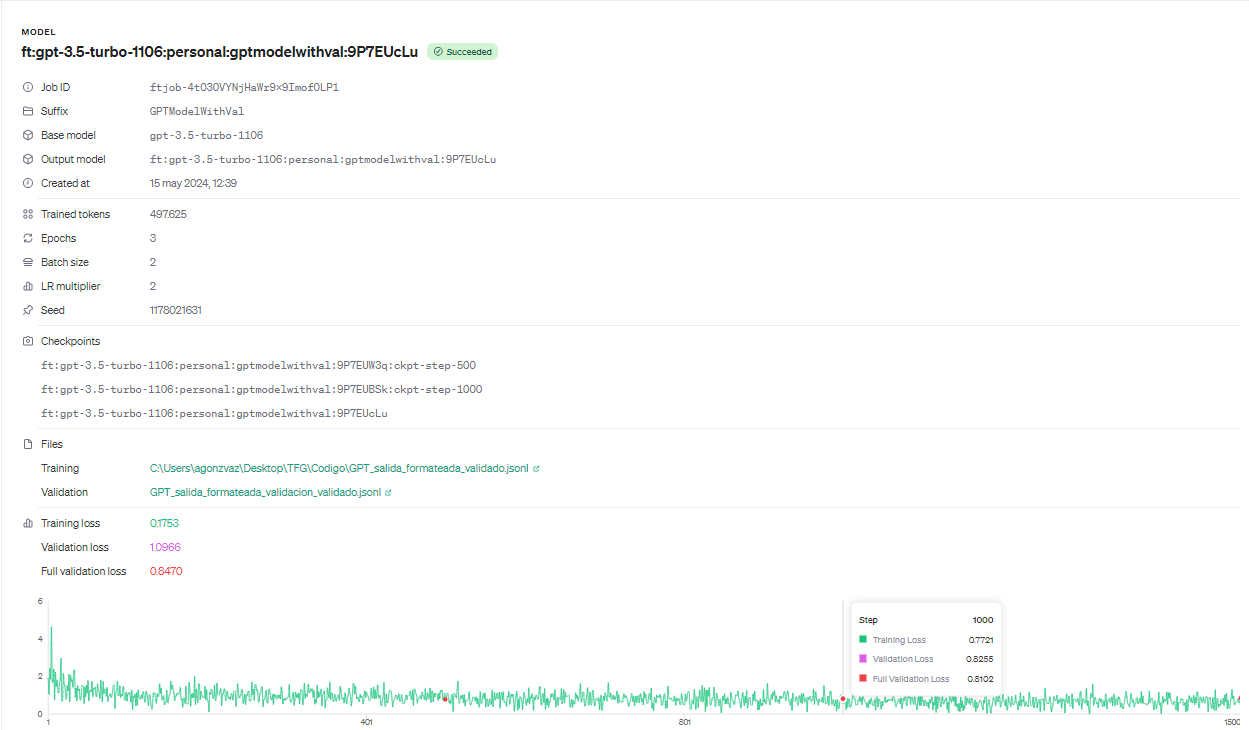
\includegraphics[width=\textwidth,keepaspectratio]{imaxes/5_GPT_EntrenamientoInterfaz.png}
  \caption{Resultado del entrenamiento GPT.}
  \label{fig:5_GPT_EntrenamientoInterfaz}
\end{figure}


\newpage % Fuerza un salto de página
Una vez finalizado el entrenamiento, el modelo puede ser evaluado y ajustado utilizando la interfaz de \acrshort{GPT}. Es posible comparar su rendimiento con otros modelos y experimentar con parámetros como la temperatura, que afecta la creatividad de las respuestas generadas, y el uso de \gls{token}s, que controla la longitud de las respuestas como se muestra en la figura \ref{fig:5_ComparativaModeloGPT}. Estos ajustes permiten optimizar el modelo según las necesidades específicas y mejorar su desempeño en diferentes contextos y aplicaciones.
\bigskip % Deja una línea en blanco

\begin{figure}[htbp!]
  \centering
  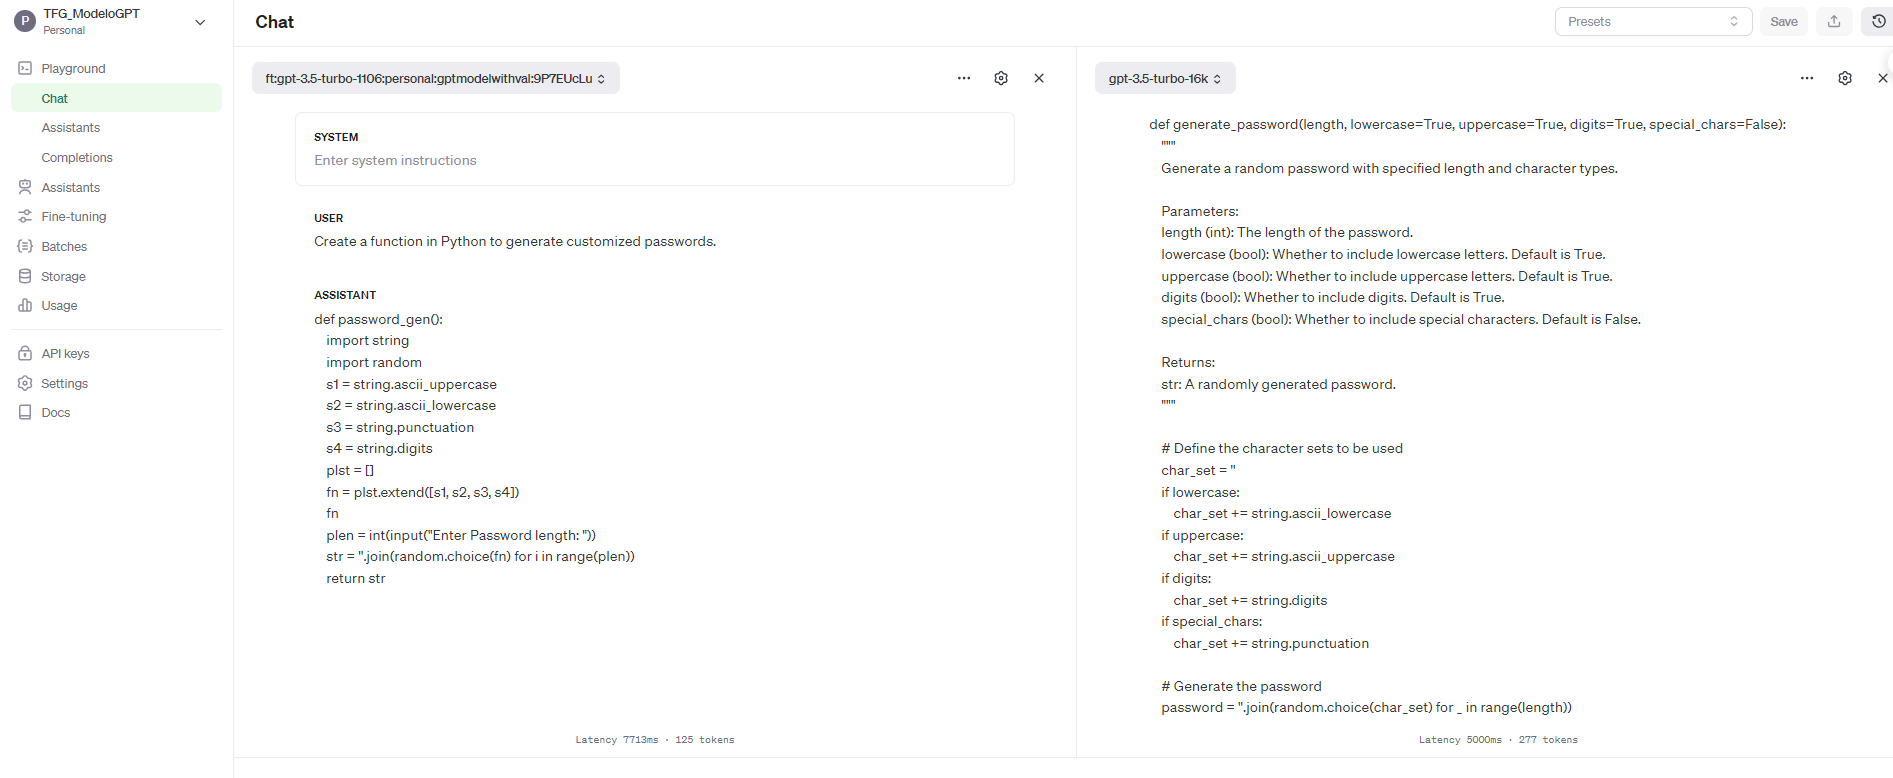
\includegraphics[width=\textwidth,keepaspectratio]{imaxes/5_ComparativaModeloGPT.png}
  \caption{Ejemplo comparativo entre el modelo entrenado y GPT-3.5-Turbo.}
  \label{fig:5_ComparativaModeloGPT}
\end{figure}

En el contexto de nuestra investigación, se identificó que el proceso de tokenización implementado durante el Fine-Tuning del modelo \acrshort{GPT} fue determinante para optimizar la eficiencia y minimizar los costos asociados. El costo total incurrido para el Ajuste Fino de nuestro modelo ascendió a 3.98 dólares \cite{APIOpenApi}, representando una alternativa considerablemente económica en comparación con el uso de modelos más avanzados, como el GPT-3.5 Turbo. La eficiente gestión de tokens facilitó ajustes precisos al modelo, evitando gastos excesivos y preservando la capacidad y robustez del \acrshort{GPT}-3.5 Turbo para su aplicación en nuestro proyecto específico.

\subsection{Modelo LLAMA}

\acrshort{LLaMA} es actualmente uno de los modelos de lenguaje más destacados, desarrollado y liberado por Meta. Similar a \acrshort{GPT}, emplea la arquitectura de Transformers \ref{subsubsec:transformers} para procesar secuencias de texto. El entrenamiento de \acrshort{LLaMA} se divide en dos fases distintas: una fase inicial de preentrenamiento, que se realiza con un extenso conjunto de ejemplos no clasificados para adquirir un conocimiento general del lenguaje, seguida de una fase de Ajuste Fino. Durante el Ajuste Fino, el modelo se especializa en tareas específicas como la clasificación o la comprensión de textos. Esta estructura de entrenamiento permite que \acrshort{LLaMA}  se adapte eficazmente a una amplia gama de aplicaciones lingüísticas, consolidando su posición como un referente en el campo de los modelos de lenguaje a gran escala.

\bigskip % Deja una línea en blanco
En nuestras evaluaciones optamos por \textbf{LLaMA 3}, un modelo recién lanzado que busca superar a sus versiones anteriores en eficiencia y rendimiento. Dos variantes de modelos \acrshort{LLaMA} 3 fueron introducidas basadas en su tamaño: el modelo de 8 mil millones de parámetros (8B) para resultados eficientes y el de 70 mil millones de parámetros (70B) diseñado para tareas complejas. Específicamente, hemos decidido utilizar la versión de \textbf{8B} utilizando el modelo \textbf{unsloth/llama-3-8b-bnb-4bit}, que se encuentra en Hugging Face (\href{https://huggingface.co/unsloth/llama-3-8b-bnb-4bit}{Enlace}).
Se eligió este modelo por su rápido proceso de carga de muestras en el entrenamiento y por las muchas opiniones positivas en el ámbito de modelos de lenguaje a gran escala.

\bigskip % Deja una línea en blanco
Para llevar a cabo este entrenamiento, hemos utilizado un archivo de \textbf{Google Colab} \cite{GoogleColab}  que se encuentra disponible en el enlace proporcionado en relación al modelo elegido anteriormente. Hemos alterado este archivo para adaptarlo a nuestros requerimientos, especialmente por las particularidades de nuestra investigación. Utilizar Google Colab nos brinda la posibilidad de trabajar en un entorno controlado, donde todas las pruebas se llevan a cabo bajo las mismas condiciones en cuanto a memoria, \acrshort{CPU} y versiones de paquetes. Esto asegura un ambiente muy propicio para llevar a cabo comparaciones entre distintos modelos.

\newpage
En primer lugar, comenzamos por la carga de información, para lo cual contamos con un archivo de entrenamiento y otro de validación, ambos en formato \acrshort{JSON}. Estos archivos son fundamentales para los tres entrenamientos que llevaremos a cabo con distintos modelos. Específicamente, \acrshort{LLaMA}  necesita que las muestras sean cargadas de acuerdo a un formato de comando particular, que incluye separadores para distinguir los mensajes y, en cada uno de ellos, el contexto de la salida relacionada.
\bigskip % Deja una línea en blanco

\begin{lstlisting}[language=Python, caption={Conversión JSON a TXT.}, label=listado3]
import json

def transform_conversation(messages):
    reformatted_segments = []

    # We start from 1 because we skip the initial system message
    for i in range(1, len(messages), 2):
        if i + 1 < len(messages) and messages[i]['role'] == 'user' and messages[i+1]['role'] == 'assistant':
            user_text = messages[i]['content']
            assistant_text = messages[i+1]['content']

            # Apply the new template
            reformatted_segments.append(f'<s>[INST] {user_text} [/INST] {assistant_text} </s>')

    return ''.join(reformatted_segments)

# Apply the transformation
transformed_texts = []
for conversation in data['messages']:
    transformed_texts.append(transform_conversation(conversation['messages']))

\end{lstlisting}

\bigskip % Deja una línea en blanco

En la ejecución de esta prueba, empleamos en Google Colab una tarjeta gráfica de aceleración, la GPU A100 de NVIDIA \cite{A100}, conocida por su alta capacidad de cómputo y eficiencia en el procesamiento de operaciones de inteligencia artificial. Este modelo de \acrshort{GPU} facilita el manejo de grandes volúmenes de datos y modelos complejos gracias a su arquitectura optimizada y a su extensa memoria, lo que nos permitió alcanzar resultados eficientes y procesar la gran cantidad de ejemplos de nuestra investigación.

\bigskip % Deja una línea en blanco

Para el ajuste del modelo, utilizamos métodos de Fine-Tuning avanzados, como \gls{QLoRA}, que nos permitió realizar una \textbf{cuantificación} eficiente hasta una precisión de 4 bits sin degradar el rendimiento del modelo. Este método se enfoca en ajustar solamente pequeños adaptadores añadidos al modelo preentrenado, lo cual implica que solo los \gls{gradiente}s de estas capas se actualizan durante el entrenamiento, manteniendo inalterado el resto del modelo congelado de 4 bits. La ventaja de este enfoque es que la \acrshort{VRAM} se utiliza de manera más eficiente y se evita la sobrecarga computacional de entrenar un modelo grande desde cero. El beneficio de esta estrategia radica en la optimización del uso de la \acrshort{VRAM} y en la reducción de la carga computacional al entrenar un modelo extenso desde cero. También, nuestros hallazgos verificaron que la precisión del modelo no se ve impactada por la cuantificación de 4 bits, lo cual confirma la efectividad de \gls{QLoRA} como enfoque de adaptación en contextos de baja precisión numérica.

\bigskip % Deja una línea en blanco

\begin{figure}[htbp!]
  \centering
  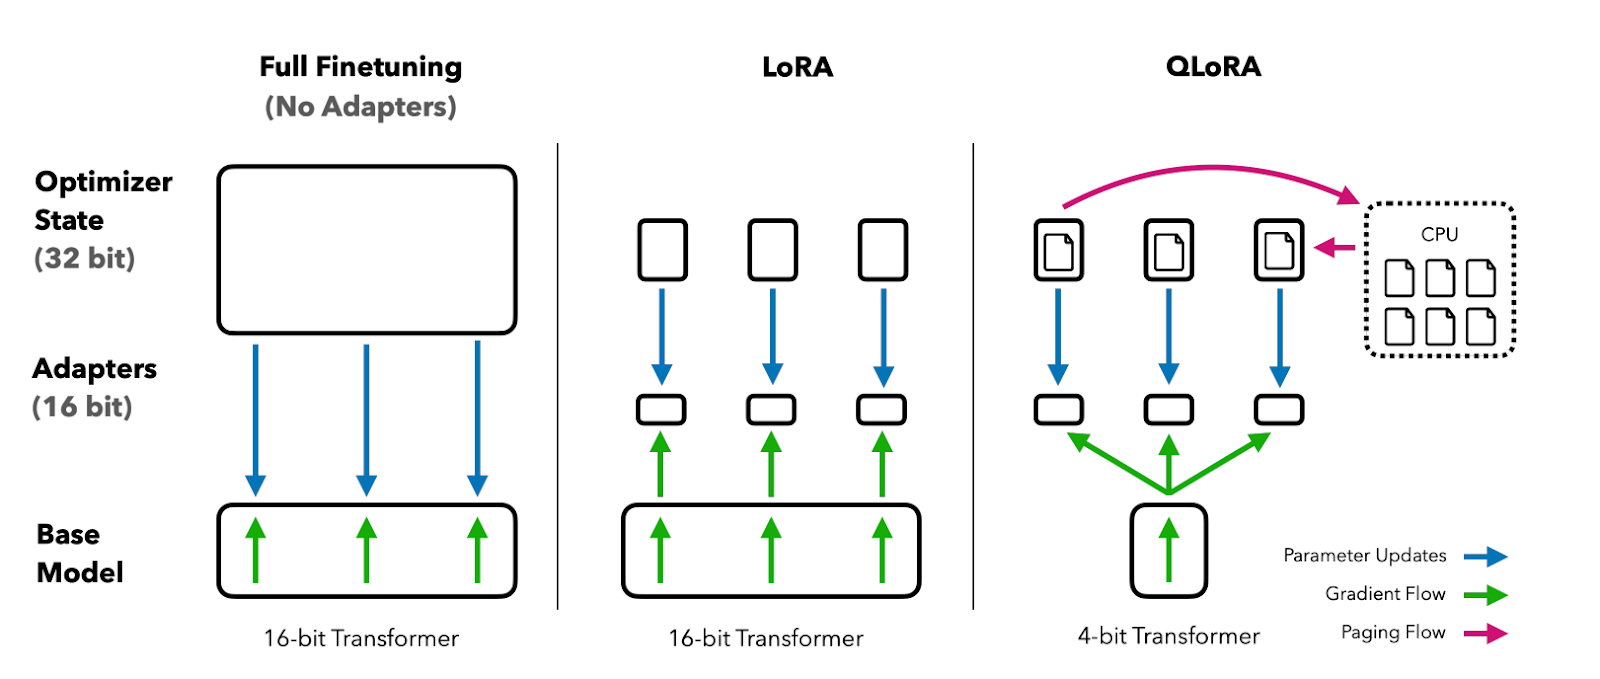
\includegraphics[width=\textwidth,keepaspectratio]{imaxes/5_QLORA.png}
  \caption[Cuantificación de 4 bits mediante QLoRA]{Cuantificación de 4 bits mediante QLoRA. \textit{Fuente: \cite{Mercity2024FineTuning}}}
  \label{fig:5_QLORA.png}
\end{figure}


\bigskip % Deja una línea en blanco

Posteriormente, continuamos con la carga del modelo y la configuración de ciertos parámetros necesarios por QLoRA para asegurar una eficiente configuración. Después, definimos los parámetros de entrenamiento. Es crucial mencionar que hemos realizado entrenamientos similares para no afectar los datos resultantes, ya que planeamos comparar otros modelos en el futuro. Para asegurar la coherencia, hemos utilizado los valores de los parámetros del modelo \acrshort{GPT} mencionados en la sección previa (ver Subsección \ref{subsec:modelogpt}). También analizaremos la utilización del gradiente, el cual será utilizado para reducir una función de pérdida que evalúa la discrepancia entre las predicciones del modelo y los valores reales, modificando los parámetros del modelo, como los pesos en una red neuronal.

\bigskip % Deja una línea en blanco

Como consecuencia, se obtiene la tabla mencionada en la referencia \ref{fig:5_LLAMA_TablaSteps.png}, la cual exhibe los resultados alcanzados en las distintas etapas del procedimiento. Este cuadro es esencial para medir el desempeño del modelo en cada etapa de entrenamiento y facilita la comparación del efecto de los cambios realizados en los parámetros.


\clearpage  % Esto fuerza a LaTeX a colocar todas las figuras pendientes y comenzar en una nueva página

\begin{figure}[htbp!]
  \centering
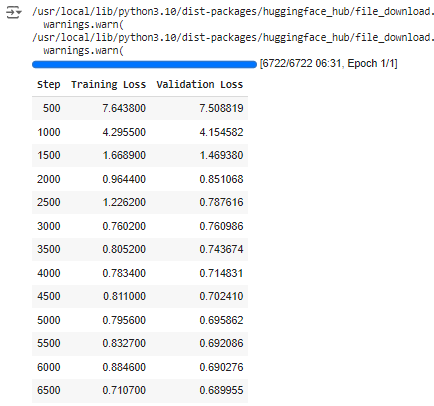
\includegraphics[width=0.8\textwidth,keepaspectratio]{imaxes/5_LLAMA_TablaSteps.png}
  \caption{Tabla con resultados del entrenamiento y validación de LLAMA 3.}
  \label{fig:5_LLAMA_TablaSteps.png}
\end{figure}

\bigskip % Deja una línea en blanco

Al igual que con \acrshort{GPT}, hemos decidido mostrar una representación visual de los resultados, incluyendo las etapas de entrenamiento y validación. Este gráfico ayuda a entender cómo se comporta el modelo a lo largo del tiempo y permite evaluar de forma más intuitiva su rendimiento en distintas etapas.

\bigskip % Deja una línea en blanco

\begin{figure}[htbp!]
  \centering
  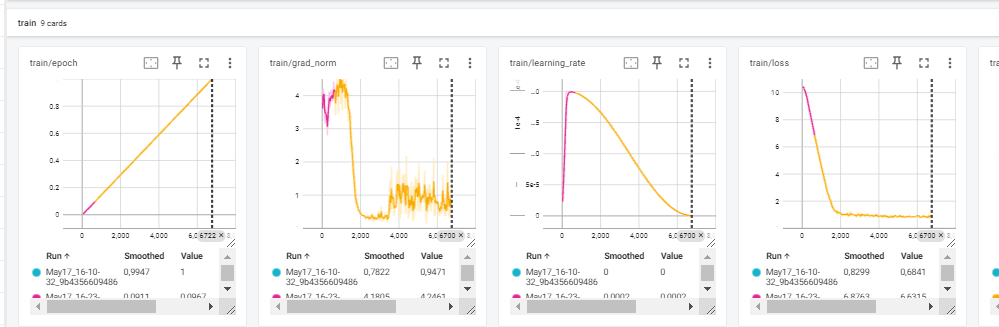
\includegraphics[width=\textwidth,keepaspectratio]{imaxes/5_LLAMA_Graficos_Train.png}
  \caption{Gráfica con los resultados del entrenamiento en LLAMA 3.}
  \label{fig:5_LLAMA_Graficos_Train.png}
\end{figure}

\bigskip % Deja una línea en blanco

Podemos observar en las secciones anteriores las diferentes gráficas \ref{fig:5_LLAMA_Graficos_Train.png} que representan diversos aspectos del entrenamiento:

\begin{itemize}
    \item \textbf{Epoch (train/epoch):} El gráfico muestra un aumento lineal en el número de epochs, lo que es esperado ya que representa el progreso del entrenamiento.

    \item \textbf{Norma del Gradiente (train/grad\_norm):} El valor de la norma del gradiente es volátil al principio pero luego se estabiliza. Altos valores iniciales y fluctuaciones pueden indicar ajustes grandes en los pesos del modelo, que luego se suavizan.

    \item \textbf{Tasa de Aprendizaje (train/learning\_rate):} La tasa de aprendizaje disminuye dramáticamente después de cierto punto, lo cual es típico de los esquemas de reducción de la tasa de aprendizaje para ayudar al modelo a converger mejor hacia el final del entrenamiento.

    \item \textbf{Loss de Entrenamiento (train/loss):} La pérdida de entrenamiento disminuye de manera constante, lo que indica un buen aprendizaje durante las \textit{epochs}. La tendencia descendente es un buen signo de que el modelo está aprendiendo adecuadamente.
\end{itemize}

\bigskip % Deja una línea en blanco

De igual forma, se pueden observar \ref{fig:5_LLAMA_Grafico_Val.png}{} los aspecto del proceso de evaluación realizado:

\begin{figure}[htbp!]
  \centering
  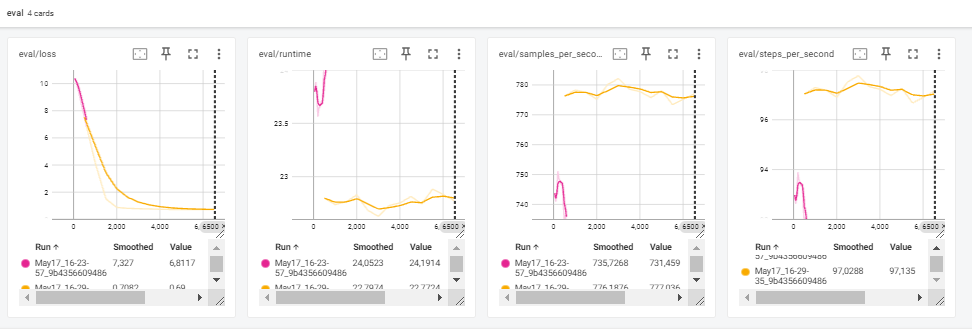
\includegraphics[width=\textwidth,keepaspectratio]{imaxes/5_LLAMA_Grafico_Val.png}
  \caption{Gráfica con los resultados de la validación de LLAMA 3.}
  \label{fig:5_LLAMA_Grafico_Val.png}
\end{figure}

\bigskip % Deja una línea en blanco

\begin{itemize}
    \item \textbf{Loss de Evaluación (eval/loss):} La pérdida disminuye significativamente y de forma estable a lo largo de las iteraciones, lo que indica que el modelo está aprendiendo y mejorando su rendimiento en los datos de validación.

    \item \textbf{Tiempo de Ejecución por Evaluación (eval/runtime):} Hay fluctuaciones en el tiempo de ejecución, pero parece estabilizarse hacia el final. No hay indicios claros de problemas como fugas de memoria que podrían aumentar el tiempo de ejecución con más iteraciones.

    \item \textbf{Muestras por Segundo (eval/samples\_per\_second):} Este valor se mantiene bastante estable, aunque hay un pico visible en la gráfica. Esto podría indicar un momento de optimización o ajuste en el proceso de evaluación.

    \item \textbf{Pasos por Segundo (eval/steps\_per\_second):} Similar a las muestras por segundo, es bastante estable, lo cual es positivo porque muestra consistencia en la velocidad de procesamiento del modelo durante la evaluación.
\end{itemize}

\bigskip % Deja una línea en blanco

El entrenamiento de \acrshort{LLaMA} 3 ha sido exitoso y eficaz, como se evidencia por la constante y notable disminución de la pérdida observada en las etapas de entrenamiento y evaluación. Esto indica que el modelo ha aprendido de manera efectiva, ya que la pérdida ha disminuido. Además, \acrshort{LLaMA} 3 ha demostrado ser estable en cuanto a su tiempo de ejecución y procesamiento. Hacer cambios en la tasa de aprendizaje y regular la norma del gradiente pueden mejorar la configuración de los parámetros para optimizar de manera efectiva. Estos hallazgos destacan que \acrshort{LLaMA} 3 es un modelo sólido y capaz, listo para ser utilizado con éxito en labores de procesamiento del lenguaje.
\bigskip % Deja una línea en blanco


Por último, debido al entorno de código abierto de este proceso de capacitación, se ha optado por compartir el modelo entrenado y los conjuntos de datos en la plataforma de Hugging Face (\href{https://huggingface.co/eibeel/llama3_python_TFG}{Enlace}) con el objetivo de respaldar y promover el desarrollo de modelos de código abierto. Esta es una muy buena alternativa para hacer pruebas con los modelos empleando herramientas como LM Studio \cite{LMStudio}, donde es posible descargar los modelos elegidos y hacer peticiones para comparar sus resultados.
\bigskip % Deja una línea en blanco

\subsection{Modelo Mixtral}

En esta sección, analizaremos nuestro proyecto utilizando \textbf{Mixtral}, un modelo de lenguaje creado por la empresa emergente francesa Mistral AI. Este proyecto fue establecido en abril de 2023 por antiguos trabajadores de Meta y Google. Indudablemente, Mixtral es uno de los modelos más prometedores en la actualidad, equiparable a \acrshort{GPT} y \acrshort{LLaMA}, y puede manejar cantidades de datos considerablemente más grandes. Mixtral se distingue por ser de código abierto.

\bigskip % Deja una línea en blanco

La estructura de entrenamiento de Mixtral es fundamental para su éxito, ya que garantiza resultados rápidos y eficientes. Esto se logra gracias al sistema \acrfull{MoE}.

\bigskip % Deja una línea en blanco

Un sistema \acrshort{MoE} \cite{MistureExperts} es una técnica utilizada en el área de los modelos de lenguaje que fragmenta un modelo extenso en múltiples submodelos más reducidos, cada uno enfocado en un conjunto particular de funciones. Esta especialización mejora la eficiencia y efectividad del sistema en la gestión de diversas tareas.

\bigskip % Deja una línea en blanco

La entrada se transforma en un vector con sus propias características \ref{fig:5_MIXTRAL_MoE}, que posteriormente se introduce en la red de enrutamiento. En este momento, es necesario determinar a cuáles modelos enviar la entrada, basándose en cuáles de ellos producirán la salida óptima. Para seleccionar, se asigna una puntuación a cada submodelo de \acrshort{MoE}, indicando su habilidad para abordar la tarea según su especialización. Una vez se obtienen estas calificaciones, el router selecciona los submodelos más competentes, aquellos con la mejor calificación, para llevar a cabo la tarea, combinando al final sus resultados para producir el resultado final, conocido como \textit{ensemble} en el campo del Machine Learning. En el nuevo modelo de Mistral, se eligen los dos modelos más competentes.

\bigskip % Deja una línea en blanco


\begin{figure}[ht!]
  \centering
  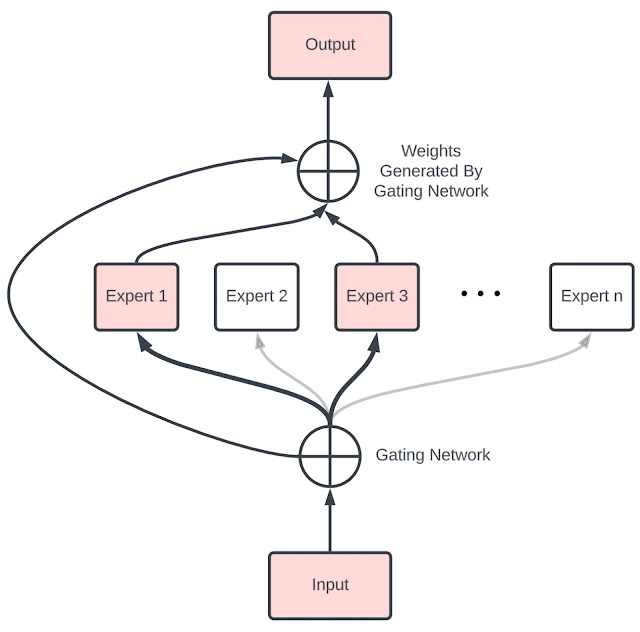
\includegraphics[width=0.5\textwidth, keepaspectratio]{imaxes/5_MIXTRAL_MoE.jpg}
  \caption[Arquitectura Mixture of Experts]{Arquitectura Mixture of Experts. \textit{Fuente: \cite{Elmo2024Mixtral}}}
  \label{fig:5_MIXTRAL_MoE}
\end{figure}



\bigskip % Deja una línea en blanco

En nuestra selección, elegimos \textbf{Mixtral-8x7B}, que salió al mercado recientemente. Es uno de los modelos de código abierto más poderosos en la actualidad, incluso comparable con los modelos destacados de OpenAI y Meta. En este momento, existen diversas variantes de Mixtral, como la modalidad con un único modelo de 7 mil millones de parámetros (más eficaz) y las modalidades con varios modelos, como las de 8x7 mil millones de parámetros y 8x22 mil millones de parámetros. Indudablemente, el ámbito open source está empezando a competir con compañías de gran tamaño. En nuestra situación, por la falta de recursos, hemos elegido trabajar con la versión de 8x7B, utilizando el modelo \textbf{mistralai/Mistral-7B-Instruct-v0.1}.

\bigskip % Deja una línea en blanco

Durante la ejecución del entrenamiento, hemos decidido utilizar Google Colab ya que permite sacar mayor provecho de los recursos disponibles en comparación con los de nuestra propia computadora portátil. Para lograrlo, hemos tomado como referencia los pasos de la sección \ref{subsec:modelogpt}, puesto que el propósito del proyecto es poder obtener conclusiones comparativas de los tres modelos en situaciones parecidas.

\bigskip % Deja una línea en blanco

Iniciamos primero con la carga de información. En esta etapa, no se han requerido efectuar cambios en los archivos de datos, ya que hemos utilizado los archivos en formato txt previamente utilizados. Mixtral no especifica un requisito en el formato del \textit{prompt}, pero sí recomienda seguir los patrones que actualmente se emplean, diferenciando el texto de usuario y el de asistente.

\bigskip % Deja una línea en blanco

El uso de \textit{padding} es frecuente en el procesamiento de \acrshort{NLP} para garantizar que todas las secuencias de entrada tengan la misma longitud. Esto es fundamental en el procesamiento por lotes, ya que es imprescindible que las secuencias tengan longitudes uniformes para que los modelos de aprendizaje automático puedan procesarlas eficazmente.

\bigskip % Deja una línea en blanco

En el caso de Mixtral, lo hemos aplicado de la siguiente forma:

\bigskip % Deja una línea en blanco

\begin{lstlisting}[language=Python, caption={Parámetro de padding.}, label=listado4]
try:
    # Attempt to load the tokenizer
    tokenizer = AutoTokenizer.from_pretrained(model_id, force_download=True)
    tokenizer.pad_token = tokenizer.unk_token
    tokenizer.pad_token_id = tokenizer.unk_token_id
    tokenizer.padding_side = 'right'
    print("Tokenizer loaded successfully.")

    # Attempt to load the model
    model = AutoModelForCausalLM.from_pretrained(model_id, force_download=True)
    print("Model loaded successfully.")
except Exception as e:
    print(f"Error loading the tokenizer or model: {e}")
\end{lstlisting}

\bigskip % Deja una línea en blanco

Es relevante destacar que utilizamos los mismos recursos que en versiones anteriores, como la tarjeta de aceleración gráfica, la \textbf{GPU A100}. Además, emplearemos la misma configuración y métodos de capacitación. Utilizando el Fine-Tuning, readoptaremos la técnica eficaz de \acrshort{QLoRA} para ajustar el modelo a una precisión de 4 bits y aumentar la eficiencia aún más.

\bigskip % Deja una línea en blanco

Después de cargar los datos y el modelo, ahora vamos a ajustar los parámetros de entrenamiento para asegurarnos de tener las mismas condiciones que en modelos previos y poder hacer comparaciones válidas.
A continuación, se presenta esta disposición para comprender minuciosamente los campos y valores asociados.

\bigskip % Deja una línea en blanco

\begin{lstlisting}[language=Python, caption={Argumentos del entrenamiento.}, label=listado5]
training_arguments = TrainingArguments(
        output_dir="./results_mixtral_sft/",
        evaluation_strategy="steps",
        do_eval=True,
        optim="paged_adamw_8bit",
        num_train_epochs=1,
        per_device_train_batch_size=4,
        gradient_accumulation_steps=2,
        per_device_eval_batch_size=4,
        log_level="debug",
        save_steps=1000,
        logging_steps=logging_steps,
        learning_rate=2e-4,
        eval_steps=500,
        max_steps=-1,
        lr_scheduler_type="linear",
        report_to="tensorboard"  
)
\end{lstlisting}

\bigskip % Deja una línea en blanco

Algunos de los argumentos anteriores con mayor relevancia son:

\begin{itemize}
    \item \textbf{Evaluation\_strategy}: Evalúa el modelo cada cierto número de pasos.
    \item \textbf{Do\_eval}: Indica si se debe realizar la evaluación durante el entrenamiento.
    \item \textbf{Num\_train\_epochs}: Número de épocas de entrenamiento.
    \item \textbf{Per\_device\_train\_batch\_size}: Tamaño del \textit{batch} de entrenamiento por dispositivo (GPU/CPU).
    \item \textbf{Gradient\_accumulation\_steps}: Número de pasos de acumulación de gradientes antes de realizar una actualización de parámetros.
    \item \textbf{Per\_device\_eval\_batch\_size}: Tamaño del \textit{batch} de evaluación por dispositivo.
    \item \textbf{Max\_steps}: Número máximo de pasos de entrenamiento. \textbf{-1} indica que no hay límite máximo de pasos, se entrenará por el número de épocas especificadas.
    \item \textbf{Lr\_scheduler\_type}: Tipo de programador de tasa de aprendizaje. "\textit{linear}" reduce la tasa de aprendizaje linealmente a lo largo del entrenamiento.
\end{itemize}


\bigskip % Deja una línea en blanco

Después de completar la capacitación, se accede a los datos de la tabla mencionada en \ref{fig:5_LLAMA_TablaSteps.png}, lo que permite visualizar los resultados en cada fase. En esa tabla se puede ver cómo funciona el modelo durante las etapas de entrenamiento y validación.

\bigskip % Deja una línea en blanco

\begin{figure}[htbp!]
  \centering
  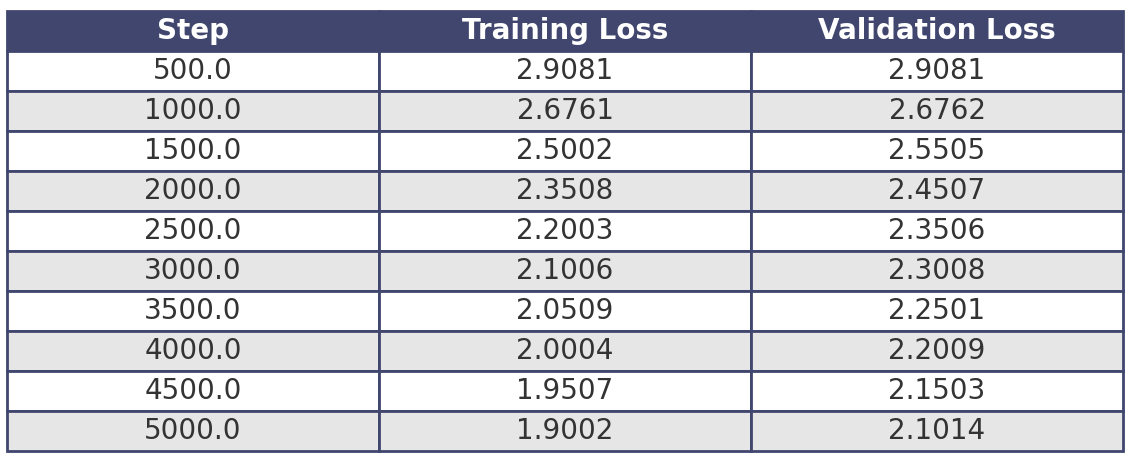
\includegraphics[width=\textwidth,keepaspectratio]{imaxes/5_MIXTRAL_TablaTeps.png}
  \caption{Tabla con resultados del entrenamiento y validación en MIXTRAL.}
  \label{fig5_MIXTRAL_TablaTeps}
\end{figure}

\bigskip % Deja una línea en blanco

Al igual que en las situaciones previas, hemos decidido mostrar de manera visual los resultados de las fases de entrenamiento y validación. Esto nos permitirá comprender la forma en que nuestro modelo se comporta frente a los datos dados.

\bigskip % Deja una línea en blanco

\begin{figure}[htbp!]
  \centering
  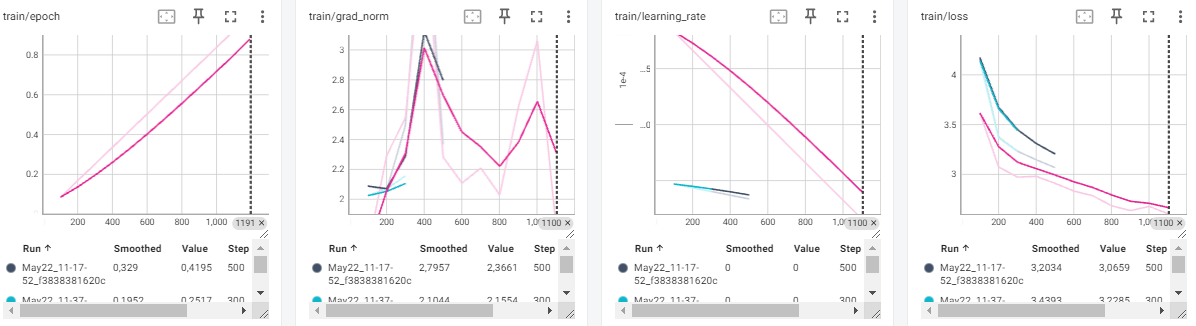
\includegraphics[width=\textwidth,keepaspectratio]{imaxes/5_MIXTRAL_Grafico_Train.png}
  \caption{Gráfica con los resultados del entrenamiento en MIXTRAL.}
  \label{fig:5_MIXTRAL_Grafico_Train}
\end{figure}

\bigskip % Deja una línea en blanco

\begin{itemize}
    \item \textbf{Epoch (train/epoch):} La evolución del entrenamiento según las épocas sigue una tendencia lineal, lo que sugiere que el modelo está adquiriendo conocimiento de forma constante a lo largo del tiempo, cumpliendo con las expectativas durante el proceso de entrenamiento.
    \item \textbf{Norma del Gradiente (train/grad\_norm):} La representación visual del gradiente de la norma presenta variaciones, con un punto más alto al principio y disminuciones después. Esta situación es típica, ya que el modelo modifica los gradientes mientras se entrena para reducir la pérdida. Los picos pueden señalar instantes en los que el modelo hizo cambios importantes en los pesos.
    \item \textbf{Tasa de Aprendizaje (train/learning\_rate):} La disminución de la tasa de aprendizaje se representa en la gráfica de forma exponencial. Una técnica habitual para garantizar que el modelo realice ajustes más precisos a medida que se acerca al mínimo de pérdida es la disminución de la tasa de aprendizaje.
    \item \textbf{Loss de Entrenamiento (train/loss):} El gráfico de la disminución de la pérdida durante el entrenamiento revela una evidente disminución, lo que sugiere una mejora en el rendimiento del modelo a lo largo del tiempo. La disminución de la pérdida se reduce rápidamente al principio y luego se estabiliza, un patrón común en el aprendizaje de modelos en las primeras etapas.
\end{itemize}

\bigskip % Deja una línea en blanco

De igual forma podemos observar \ref{fig:5_MIXTRAL_Grafico_Val} el proceso de evaluación realizado:

\bigskip % Deja una línea en blanco

\begin{figure}[htbp!]
  \centering
  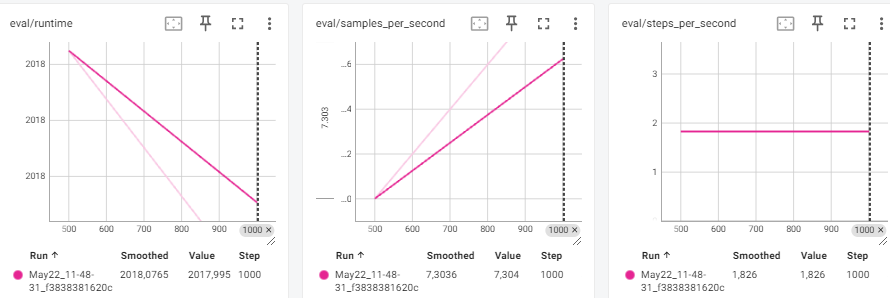
\includegraphics[width=\textwidth,keepaspectratio]{imaxes/5_MIXTRAL_Grafico_Val.png}
  \caption{Gráfica con los resultados de la validación en MIXTRAL.}
  \label{fig:5_MIXTRAL_Grafico_Val}
\end{figure}

\bigskip % Deja una línea en blanco

\begin{itemize}
    \item \textbf{Tiempo de Ejecución por Evaluación (eval/runtime):} Esto sugiere que la eficacia del proceso de validación está mejorando con el tiempo, probablemente gracias a mejoras internas y estabilidad en las fases finales del entrenamiento.
    \item \textbf{Muestras por Segundo (eval/samples\_per\_second):} Esto indica que el modelo está progresando en cuanto a eficiencia de procesamiento, siendo capaz de procesar una mayor cantidad de datos en menos tiempo a medida que avanza el entrenamiento.
    \item \textbf{Pasos por Segundo (eval/steps\_per\_second):} Esto indica una consistencia positiva en el desempeño del modelo durante la validación, lo cual es un buen signo de estabilidad.
\end{itemize}

\bigskip % Deja una línea en blanco

Según las gráficas (\ref{fig:5_MIXTRAL_Grafico_Train} y \ref{fig:5_MIXTRAL_Grafico_Val}) y la tabla (\ref{fig:5_LLAMA_TablaSteps.png}), se sugiere que el modelo \textbf{MIXTRAL} ha sido entrenado de manera eficiente, logrando reducir el tiempo de ejecución y aumentar la velocidad de procesamiento de las muestras. Esto señala un proceso de entrenamiento y validación optimizado. La disminución de la pérdida en entrenamiento y validación es constante, lo que sugiere que el modelo está aprendiendo de manera efectiva y generalizando correctamente a los datos de validación. Asimismo, la regla del gradiente y la velocidad de aprendizaje presentan comportamientos predecibles que favorecen la convergencia del modelo, y la consistencia en los pasos por segundo durante la validación respalda esta afirmación. En resumen, parece que el entrenamiento del modelo MIXTRAL fue efectivo, demostrando un buen desempeño y estabilidad durante cada etapa, indicando una optimización eficiente en el procesamiento de datos.

\bigskip % Deja una línea en blanco.

Por último, llevar a cabo pruebas en este proyecto de código abierto sugiere que proyectos como \acrshort{GPT} y \acrshort{LLaMA} no están muy lejos en comparación con MIXTRAL. De la misma manera que hicimos en ejemplos anteriores, pondremos tanto el modelo entrenado como los datos empleados en la plataforma de Hugging Face (\href{https://huggingface.co/eibeel/mixtral_tfg}{Enlace}) para continuar contribuyendo al desarrollo de software de código abierto.


\subsection{Evaluación de modelos y comparativa de resultados}
\label{subsec:evaluaciónmodelos}

En esta sección examinaremos los resultados de los modelos con métricas y métodos diferentes para determinar cuál es el más adecuado para nuestras necesidades. La valoración y el estudio de modelos, como \acrshort{GPT}, \acrshort{LLaMA} y MIXTRAL, son fundamentales en inteligencia artificial para garantizar su eficacia y exactitud en funciones como la redacción de texto, traducción automática, síntesis de textos y resolución de preguntas.

\bigskip % Deja una línea en blanco.

Una investigación reciente \cite{hassid2024larger} indica que modelos con menos parámetros (7 mil millones y 13 mil millones) pueden ser más efectivos que modelos con más parámetros (34 mil millones y 70 mil millones) en tareas de generación de código con el mismo costo computacional. En este \acrshort{TFG}, utilizaremos medidas como \acrshort{BLEU} y ROUGE para valorar los modelos, investigando si la repetición de la ejecución de modelos pequeños podría ser más efectiva que el empleo de modelos grandes.

\bigskip % Deja una línea en blanco

Primero, optamos por llevar a cabo varios experimentos con las predicciones de los modelos ensayados. Para ello, damos a nuestros modelos un \textit{prompt} que indica lo requerido y la respuesta deseada. De acuerdo a las especificaciones de cada modelo, podremos notar las disparidades entre ellos y tener una clara noción de cuál es el más adecuado para nuestro problema.

\bigskip % Deja una línea en blanco

\begin{lstlisting}[language=Python, caption={Prompt y salida de referencia.}, label=listado6]
def main():
    # Prompt para generar el código Python
    prompt = "Write a Python function that sums all prime numbers from 1 to 1000."

    # Generar predicción
    candidate = generate_predictions(model, prompt)
    print(f"Generated code:\n{candidate}")

    # Respuesta de referencia esperada (en inglés)
    reference = """
def sum_primes():
    def is_prime(n):
        if n <= 1:
            return False
        for i in range(2, int(n**0.5) + 1):
            if n % i == 0:
                return False
        return True

    total = sum(n for n in range(2, 1001) if is_prime(n))
    return total

print(sum_primes())
""".strip()

\end{lstlisting}

\bigskip % Deja una línea en blanco

A continuación, se presentará la salida producida por cada modelo con el fin de visualizar las disparidades entre ellos. Claramente, cada modelo exhibe sus propias características al abordar la cuestión que hemos planteado a través del \textit{prompt}.
\begin{itemize}
    \item \textbf{\acrshort{GPT}}: 

    \begin{lstlisting}[language=Python, caption={Salida generada por GPT.}, label=listado7]
    def isPrime(n):
        if(n<2): return False
        if(n==2): return True
        if(n%2==0): return False
        for i in range(3,int(n**0.5)+1,2):
            if(n%i==0):
                return False            
        return True

    def sum_primes(n):
     return sum([i for i in range(n + 1) if isPrime(i)])

    sum_primes(1000)
    \end{lstlisting}

    
    \item \textbf{\acrshort{LLaMA}}:

    \begin{lstlisting}[language=Python, caption={Salida generada por LLaMA.}, label=listado8]
    def sum_primes(n):
        def is_prime(num):
            if num < 2:
            return False
            for i in range(2, int(num**0.5) + 1):
                if num % i == 0:
            return False
            return True

        return sum(i for i in range(2, n+1) if is_prime(i))

    print(sum_primes(1000))
    \end{lstlisting}
    
\item \textbf{MIXTRAL}:

    \begin{lstlisting}[language=Python, caption={Salida generada por MIXTRAL.}, label=listado9]
    def sum_primes():
        def is_prime(n):
            if n <= 1:
                return False
            for i in range(2, int(n**0.5) + 1):
                if n % i == 0:
                    return False
return True

total = sum(n for n in range(2, 1001) if is_prime(n))
        return total

    print(sum_primes())
    \end{lstlisting}
\end{itemize}

Para asegurar una revisión detallada del modelo, establecimos medidas como exactitud, recordatorio, puntuación F1 y \acrshort{BLEU}. Estas medidas nos dan un valor numérico del desempeño del modelo en actividades concretas, lo que nos habilita para cotejar distintos modelos o modificaciones de hiperparámetros.

\begin{itemize}

\item\textbf{Precisión (Precision):} Este indicador evalúa la fracción de predicciones positivas acertadas de todas las predicciones positivas hechas por el modelo. En otras palabras, la precisión mide la cantidad de elementos clasificados como positivos que son verdaderamente positivos. Se estima con la fórmula:
    
\[
\text{Precisión} = \frac{\text{Verdaderos Positivos}}{\text{Verdaderos Positivos} + \text{Falsos Positivos}}
\]

    En un caso de clasificación binaria, la precisión indica cuántos de los casos identificados como positivos por el modelo son realmente positivos.

    \bigskip % Deja una línea en blanco

\item \textbf{Recuperación (Recall):} Esta métrica evalúa cuántos ejemplos positivos son identificados correctamente por el modelo en comparación con el total de ejemplos positivos presentes en el conjunto de datos. En otras términos, la recuperación indica la cantidad de elementos positivos reales que fueron correctamente reconocidos por el modelo. La fórmula se utiliza para el cálculo.
    
\[
\text{Recuperación} = \frac{\text{Verdaderos Positivos}}{\text{Verdaderos Positivos} + \text{Falsos Negativos}}
\]
    
En el caso de un problema de detección de correo no deseado, la recuperación nos proporcionará información sobre la cantidad de correos electrónicos identificados como correo no deseado por el modelo en comparación con todos los correos no deseados en el conjunto de datos.

\bigskip % Deja una línea en blanco
    
\item \textbf{Puntuación F1 (F1 Score):} Esta métrica combina la exactitud y la recuperación en un solo valor que brinda una evaluación más equilibrada de la eficacia del modelo. Resulta especialmente beneficioso cuando existe una falta de equilibrio en la distribución de clases en los datos. La F1 score se calcula como el promedio armónico de precisión y recall, y se define mediante esta fórmula:
\[
\text{Puntuación F1} = 2 \times \frac{\text{Precisión} \times \text{Recuperación}}{\text{Precisión} + \text{Recuperación}}
\]

La puntuación F1 alcanza su mejor valor en 1 (indicando una precisión perfecta y una recuperación perfecta) y su peor valor en 0 (indicando un rendimiento pobre en ambas métricas). Esta métrica es útil cuando nos interesa encontrar un equilibrio entre la precisión y la recuperación en la evaluación del modelo.

\bigskip % Deja una línea en blanco

\item \textbf{\acrfull{BLEU}:} Es una métrica utilizada para evaluar la calidad de texto generado automáticamente, como traducciones automáticas, comparándolo con una o más traducciones de referencia realizadas por humanos. BLEU mide la precisión de n-gramas, es decir, secuencias de palabras de longitud n, para ver cuántos de los n-gramas en el texto generado aparecen también en el texto de referencia. Para ello, se emplea la siguiente fórmula:


\begin{equation}
BLEU = BP \cdot \exp \left( \sum_{n=1}^{N} w_n \log p_n \right)
\end{equation}

\begin{itemize}
    \item \textbf{BP} es la penalización por longitud (Brevity Penalty).
    \item \( N \) es el máximo tamaño de los n-gramas (usualmente hasta 4).
    \item \( w_n \) es el peso asignado a la precisión de n-gramas de tamaño \( n \) (comúnmente iguales para todos los n-gramas).
    \item \( p_n \) es la precisión de los n-gramas de tamaño \( n \).
\end{itemize}

Por lo tanto, \acrshort{BLEU} es un número entre cero y uno que mide la similitud del texto traducido de manera automática con un conjunto de traducciones de referencia de alta calidad.

\end{itemize}

En nuestro estudio, una vez hemos realizado los entrenamientos con los diferentes modelos hemos obtenido una serie de resultados en función de como había sido el entrenamiento (secciones anteriores). Llegados a este punto, hemos decidido realizar un análisis más profundo respecto a la evaluación de los modelos, por lo que nos hemos centrado en las métricas comentadas anteriormente. Para la realización de este proceso hemos creado un único conjunto de datos que le hemos pasado a los diferentes modelos para obtener mayor información respecto al entrenamiento.

\bigskip % Deja una línea en blanco

En la investigación, después de completar los entrenamientos con los distintos modelos, hemos conseguido una variedad de resultados basados en la forma en que se llevó a cabo el entrenamiento. En este punto, hemos optado por llevar a cabo un examen más detallado sobre la evaluación de los modelos, enfocándonos en las métricas previamente mencionadas. Para llevar a cabo este procedimiento, hemos desarrollado un único \textit{script} que hemos proporcionado a los diversos modelos con el fin de obtener más datos sobre el proceso de entrenamiento.

\bigskip % Deja una línea en blanco

El \textit{script} consta de lo siguiente, a mayores de las librerías propias de cada modelo como pueden ser la de OpenAI o Huggin Face:

\bigskip % Deja una línea en blanco

\begin{lstlisting}[language=Python, caption={Script de evaluación del modelo.}, label=listado10]
import nltk
from nltk.translate.bleu_score import sentence_bleu, SmoothingFunction
from sklearn.metrics import precision_score, recall_score, f1_score

def generate_predictions(model, prompt):
    response = openai.Completion.create(
        model=model,
        prompt=prompt,
        max_tokens=150
    )
    prediction = response.choices[0].text.strip()
    return prediction

def calculate_bleu(references, candidates):
    smooth = SmoothingFunction().method1
    bleu_scores = [sentence_bleu([ref.split()], cand.split(), smoothing_function=smooth) for ref, cand in
                   zip(references, candidates)]
    average_bleu = sum(bleu_scores) / len(bleu_scores)
    return bleu_scores, average_bleu

def calculate_classification_metrics(y_true, y_pred):
    precision = precision_score(y_true, y_pred, average='weighted')
    recall = recall_score(y_true, y_pred, average='weighted')
    f1 = f1_score(y_true, y_pred, average='weighted')
    return precision, recall, f1

\end{lstlisting}

\bigskip % Deja una línea en blanco

A partir del \textit{script} anterior, se presenta la tabla \ref{tab:ComparacionModelos} para facilitar la visualización de los resultados y realizar análisis de los diferentes modelos evaluados.

\bigskip % Deja una línea en blanco

\begin{table}[ht!]
  \centering
  \scalebox{0.90}{ % Cambia el valor 0.90 para ajustar el tamaño
    \rowcolors{2}{white}{gray!25}
    \begin{tabular}{c|c|c|c|c}
      \rowcolor{pink!25}
      \textbf{Modelos} & \textbf{Precision} & \textbf{Recall} & \textbf{F1 Score} & \textbf{\acrshort{BLEU}} \\\hline
      Modelo \acrshort{GPT} & 0.600 & 0.600 & 0.600 & 0.700 \\
      Modelo \acrshort{LLaMA} & 0.486 & 0.486 & 0.486 & 0.568 \\
      Modelo MIXTRAL & 0.857 & 0.857 & 0.857 & 0.943 \\
    \end{tabular}
  }
  \caption{Tabla de comparación de modelos.}
  \label{tab:ComparacionModelos}
\end{table}

\bigskip % Deja una línea en blanco

Al examinar la tabla mencionada \ref{tab:ComparacionModelos}, la comparación entre los modelos proporciona datos significativos sobre su eficacia durante la fase de entrenamiento. Así que analizaremos cada métrica y hablaremos sobre las conclusiones que podemos extraer de ellas.

\bigskip % Deja una línea en blanco

En cuanto a la \textbf{\textit{precision}}, que mide la correcta clasificación de las instancias, se puede notar que el modelo MIXTRAL logra un alto porcentaje de aciertos. Además, \acrshort{GPT} muestra un nivel de rendimiento moderado, mientras que \acrshort{LLaMA} tiene un desempeño significativamente inferior en comparación con los otros modelos.

\bigskip % Deja una línea en blanco

Con respecto al \textbf{\textit{recall}}, que se refiere a la habilidad de un modelo de clasificación para reconocer de manera correcta las instancias positivas, MIXTRAL se destaca como el modelo superior. Igualmente, tanto \acrshort{GPT} como \acrshort{LLaMA} tienen aún mucho espacio para mejorar en la métrica mencionada anteriormente.

\bigskip % Deja una línea en blanco

Otra consideración importante es el \textbf{\textit{F1 Score}}, que en esencia refleja la combinación de las dos mencionadas anteriormente, siendo MIXTRAL aún el líder seguido por \acrshort{GPT} y \acrshort{LLaMA}.

\bigskip % Deja una línea en blanco

Al final, contamos con \textbf{\acrshort{BLEU}}, el cual se calcula comparando la salida generada con la salida esperada. En esta etapa, MIXTRAL muestra un buen desempeño al ser similar al código deseado, mientras que \acrshort{GPT} también genera un código que se asemeja razonablemente al de referencia, aunque con algunas discrepancias. Posteriormente, \acrshort{LLaMA} es el menos parecido en código.

\bigskip % Deja una línea en blanco

En consecuencia, al analizar las métricas se demuestra que el \textbf{Modelo MIXTRAL} destaca sobre \acrshort{GPT} y \acrshort{LLaMA} en todas las áreas evaluadas, siendo el más idóneo para la generación de código Python. Las disparidades en el desempeño de los modelos pueden ser explicadas por elementos como la calidad y cantidad de datos de entrenamiento, la estructura del modelo y las estrategias de entrenamiento empleadas. Para este trabajo en concreto, optar por MIXTRAL garantizaría los resultados más óptimos en cuanto a precisión, recall, F1 Score y semejanza con el código de referencia.

\bigskip % Deja una línea en blanco

Una vez obtengamos esta solución como resultado de nuestros análisis, vamos a comparar la información con diferentes investigaciones.

\bigskip % Deja una línea en blanco

El primer estudio \cite{estudio1} que analizamos compara diferentes \acrfull{LLMs} en su desempeño para generar código, empleando el benchmark HumanEval. Se plantea un modelo de agente múltiple que utiliza múltiples \acrshort{LLMs} para crear y analizar código de forma sistemática. En el \acrshort{GPT}-3.5 Turbo sobresale en comparación con Google Bard, \acrshort{LLaMA} y Hugging Face; sin embargo, es posible que para la generación de código en Python, MIXTRAL sea una opción recomendable.

\bigskip % Deja una línea en blanco

El estudio \cite{estudio2} investiga la habilidad de los \acrshort{LLMs} para crear programas de Python con el uso de \textit{\gls{few-shot learning}}. Se investiga cómo los modelos de mayor tamaño pueden incrementar su desempeño mediante un Ajuste Fino adecuado. Se plantea que modelos como \acrshort{GPT}-3.5 Turbo y Copilot son efectivos en general, pero optamos por MIXTRAL debido a su excelente rendimiento en Python, que es crucial para nuestra aplicación. La evaluación detallada y los criterios específicos utilizados respaldan nuestra conclusión de que MIXTRAL es el modelo más adecuado para generación de código Python.

\bigskip % Deja una línea en blanco

En resumen, los tres modelos son buenos ejemplos de \acrshort{LLMs}, simplemente algunos se adaptan mejor a un problema que otros. Según los estudios revisados, \acrshort{GPT}-3.5 Turbo se destaca como una excelente solución para una amplia variedad de problemas, gracias al extenso conjunto de datos con el cual ha sido entrenado. Aún así, llegamos a la conclusión de que \textbf{Mixtral} destaca frente a otros \acrshort{LLMs}, debido a su gran capacidad de adaptación para la creación de código \cite{MixtralWebOficial}, además de destacar por su eficacia y rentabilidad

\bigskip % Deja una línea en blanco

A continuación, se presenta una tabla comparativa entre MIXTRAL y otros \acrshort{LLMs} en base a distintos \textit{benchmarks} \ref{fig:5_TablaComparativa}.

\bigskip % Deja una línea en blanco

\begin{figure}[htbp!]
  \centering
  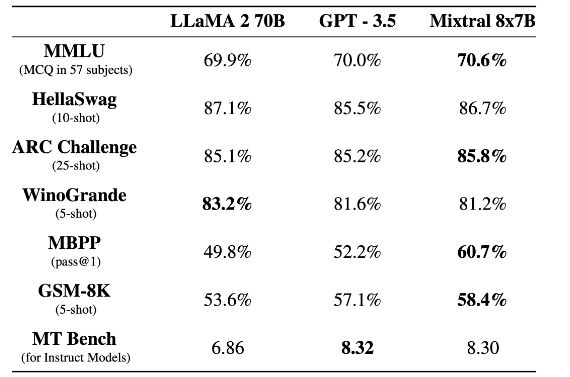
\includegraphics[width=0.75\textwidth,keepaspectratio]{imaxes/5_TablaComparativa.png}
  \caption[Tabla comparativa de modelos]{Tabla comparativa de modelos. \textit{Fuente: \cite{MixtralWebOficial}}}
  \label{fig:5_TablaComparativa}
\end{figure}
``

\section{Alternativa al Fine-Tuning: RAG}

Los sistemas que utilizan \acrshort{RAG} (ver la sección \ref{subsubsec:enfoquerag}), al incorporar fuentes externas de información, se facilita a los modelos generar respuestas más precisas y relevantes. De esta manera, no se requiere volver a entrenar el modelo; en su lugar, se utiliza la información contextual proporcionada durante la generación para ofrecer una respuesta mejorada.

\bigskip % Deja una línea en blanco

En este instante es cuando un sistema \acrshort{RAG} entra en acción. Cuando un usuario hace una búsqueda, el sistema encuentra los documentos internos más importantes y los incluye en la búsqueda al \acrshort{LLMs}. Este tipo de consulta mejorada ayuda al \acrshort{LLMs} a generar respuestas más precisas y educadas, evitando la necesidad de entrenar de nuevo. Asimismo, la posibilidad del sistema de mencionar la fuente en la que se fundamenta su respuesta aumenta la confianza de los usuarios al proporcionar un mayor nivel de fiabilidad.

\bigskip % Deja una línea en blanco

En primer lugar, es necesario transferir la información a nuestro sistema, la cual puede consistir en documentos de texto de diversos tipos y formatos (PDFs de artículos de investigación, HTML de páginas web, archivos en Markdown de una Wiki interna, tickets en un sistema de organización de trabajo, etc.). Hemos decidido usar el archivo de datos \acrshort{JSON} en nuestro sistema, el cual ya ha sido utilizado previamente en diversas secciones para entrenar distintos modelos.

\bigskip % Deja una línea en blanco

En esta etapa, optamos por dividir el texto en fragmentos, también llamados \textit{chunks}, separando así los documentos extensos en secciones más manejables. Esto es importante porque los \textit{\gls{embeddings}} tienen capacidad limitada para representar significado en forma vectorial. Al incluir y organizar estos fragmentos más pequeños en lugar de documentos completos, el sistema puede encontrar y obtener de manera más precisa las secciones más importantes para las consultas de los usuarios. En nuestra iniciativa, hemos procedido de la manera siguiente.

\bigskip % Deja una línea en blanco

\begin{lstlisting}[language=Python, caption={Fragmentación de texto.}, label=listado11]
from langchain.text_splitter import CharacterTextSplitter

text_splitter = CharacterTextSplitter(
    chunk_size=7500, chunk_overlap=100
)
doc_splits = text_splitter.split_documents(docs_list)

# Verificar el contenido de los splits
for split in doc_splits:
    print(split.page_content, split.metadata)

\end{lstlisting}

\bigskip % Deja una línea en blanco

La división de texto asegura que la información importante esté bien organizada al crear el \textit{prompt} para el modelo generativo.

\bigskip % Deja una línea en blanco

Alcanzado este punto, es necesario iniciar la búsqueda; por lo tanto, es crucial comprender el funcionamiento de los \gls{embeddings}. Cada palabra, frase, párrafo, o documento de cierta longitud se asigna a un vector numérico en un espacio de representación donde el texto se considera 'embebido'.

\bigskip % Deja una línea en blanco

\begin{figure}[htbp!]
  \centering
  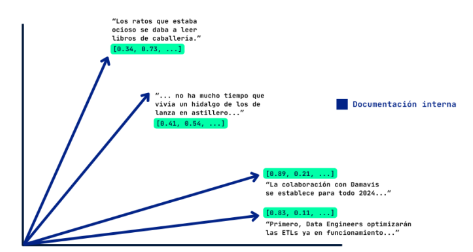
\includegraphics[width=\textwidth,keepaspectratio]{imaxes/5_RAG_Embeddingpng.png}
  \caption[Esquema vectorial del modelo embedding]{Esquema vectorial del modelo embedding. \textit{Fuente: \cite{embedding}}}
  \label{fig:5_RAG_Embedding}
\end{figure}


\bigskip % Deja una línea en blanco

El modelo de \textit{embedding} será adecuado si textos semánticamente relacionados se asignan a vectores que sean cercanos \ref{fig:5_RAG_Embedding}. Estos textos salen fragmentados con una longitud fija, la cual pasarán a llamarse nodos, donde posteriormente, a partir de un modelo \textit{embedding} y el nodo, se calculan los vectores. Donde posteriormente pasarán a almacenarse en bases de datos especialmente diseñadas para vectores de gran cantidad de componentes, que los guardan haciendo una gestión eficiente de la memoria y permitiendo, a través de distintas técnicas de indexado, mejorar la eficiencia de la búsqueda de vectores vecinos.

\bigskip % Deja una línea en blanco

En el caso que estamos estudiando, decidimos emplear el modelo de \textit{embedding} de código libre \textbf{nomic-embed-text-v1} \cite{Nomic}, el cual nos brinda acceso a una \acrshort{API} gratuita de 1 millón de tokens. En su lugar, podríamos haber optado por utilizar diferentes \textit{embeddings} más distintivos, como los de OpenAI, como por ejemplo text-embedding-ada-002, que tiene un costo asociado. Además, elegimos \textbf{ChromaDB} \cite{Chroma} como base de datos vectorial debido a su potencia y versatilidad para manejar y consultar \textit{embeddings}, mejorando las capacidades de búsqueda semántica y recuperación de datos en aplicaciones avanzadas de inteligencia artificial. En la figura \ref{fig:5_RAG_Esquema} se presenta un esquema de la configuración del procedimiento que estamos ejecutando.

\bigskip % Deja una línea en blanco

\begin{figure}[htbp!]
  \centering
  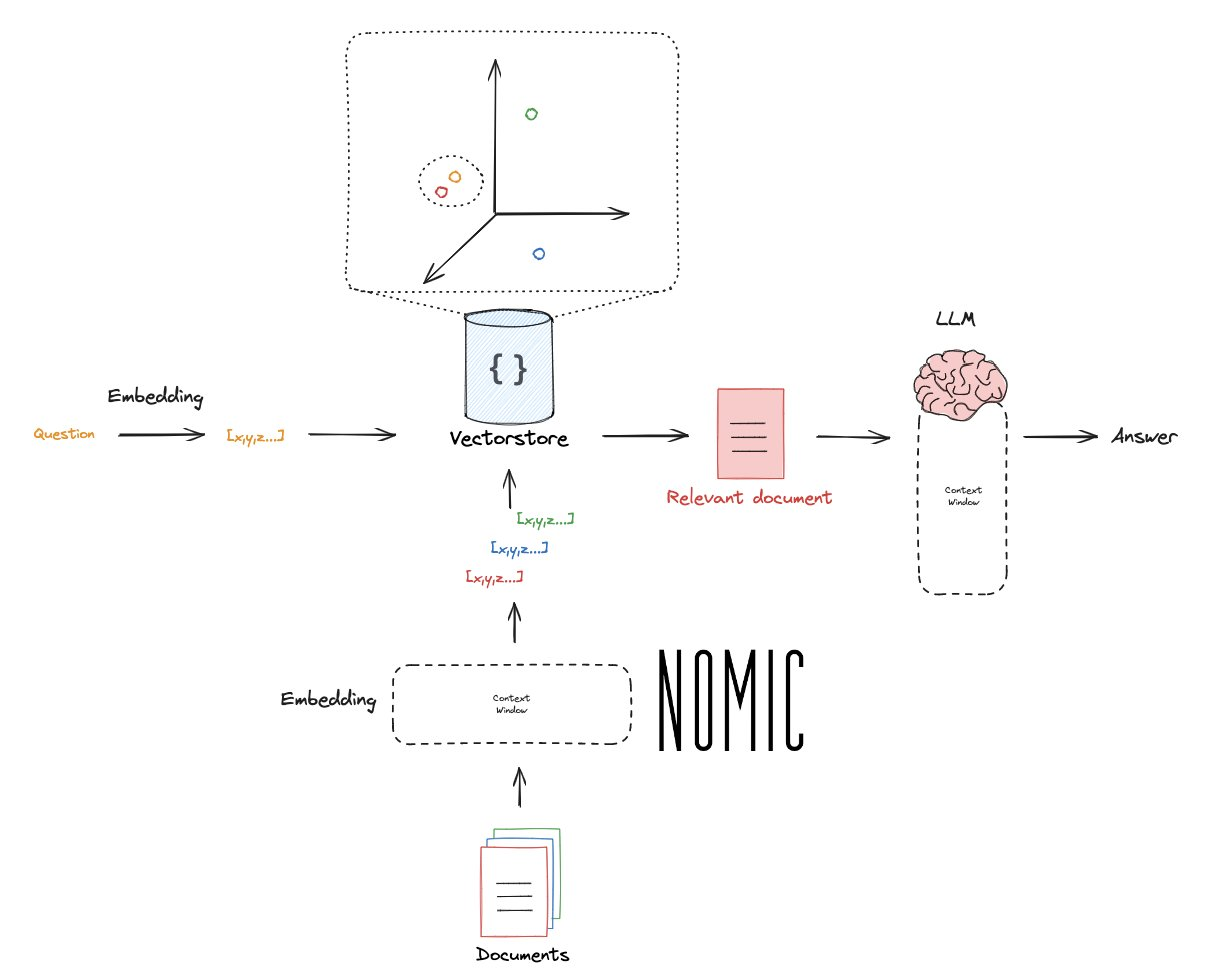
\includegraphics[width=0.85\textwidth,keepaspectratio]{imaxes/5_RAG_Esquema.jpeg}
  \caption[Esquema del proceso RAG]{Esquema del proceso RAG. \textit{Fuente: \cite{LangChainAI2023}}}
  \label{fig:5_RAG_Esquema}
\end{figure}


\bigskip % Deja una línea en blanco

En esta etapa, nos situamos en la fase de generación, en la cual podremos crear una respuesta basada en los \textit{prompts} incluidos en el archivo de entrada. Usaremos el mismo modelo que hemos estado utilizando en esta investigación, que es el \textbf{gpt-3.5-turbo} de OpenAI. Indudablemente, uno de los modelos más idóneos para satisfacer las características de nuestro proyecto.

\bigskip % Deja una línea en blanco

Al igual que hicimos con el enfoque Fine-Tuning, hemos optado por llevar a cabo un conjunto de métricas en el proceso para evaluar la eficacia de este sistema \acrshort{RAG} en nuestra iniciativa. Las métricas utilizadas son las mismas que se mencionaron anteriormente (subsección \ref{subsec:evaluaciónmodelos}), por lo que podemos tener una idea general de los resultados anticipados.

\bigskip % Deja una línea en blanco

\begin{table}[ht!]
  \centering
  \scalebox{0.90}{ % Cambia el valor 0.90 para ajustar el tamaño
    \rowcolors{2}{white}{gray!25}
    \begin{tabular}{c|c|c|c|c}
      \rowcolor{pink!25}
      \textbf{Modelos} & \textbf{Precisión} & \textbf{Recall} & \textbf{F1 Score} & \textbf{\acrshort{BLEU}} \\\hline
      RAG - Modelo GPT & 0.909& 0.909 & 0.909 & 0.032 \\
    \end{tabular}
  }
  \caption{Tabla resultados de métricas de GPT con RAG.}
  \label{tab:TablaMetricas}
\end{table}

\bigskip % Deja una línea en blanco

Basándonos en los resultados previos presentados \ref{tab:TablaMetricas}, podemos inferir las siguientes conclusiones:

\bigskip % Deja una línea en blanco

\begin{itemize}
    \item \textbf{Precisión (Precision)}: El 90.9\% de las predicciones positivas hechas por el modelo fueron precisas. Esto señala que el modelo es bastante preciso y tiene una tasa baja de falsos positivos.
    \item \textbf{Recuperación (Recall):} El 90.9\% de las instancias realmente positivas fueron identificadas correctamente por el modelo. Esto indica que el modelo puede recuperar la mayor parte de los casos importantes, presentando una tasa baja de falsos negativos.
    \item \textbf{Puntuación F1 (F1 Score):} El F1 Score representa la combinación armónica de la precisión y el recall, siendo en este caso 0.909. Esto señala un balance apropiado entre precisión y recall, lo cual es deseado en una tarea donde ambas métricas tienen la misma importancia.
    \item \textbf{\acrfull{BLEU}:} En comparación con las otras métricas, la puntuación BLEU es notablemente inferior. Un score de 0.032 indica que, a pesar de la precisión y el buen recall del modelo para identificar las categorías correctas, la generación de texto puede no coincidir de forma efectiva con el texto de referencia en términos de fluidez y coherencia.
\end{itemize}

\bigskip % Deja una línea en blanco

El rendimiento del modelo \acrshort{RAG} con \acrshort{GPT}-3.5 Turbo en términos de precisión y recall es extraordinario, logrando un 90.9\% en ambos aspectos, lo que demuestra su eficacia en la identificación y clasificación precisa de elementos relevantes. No obstante, el bajo puntuaje \acrshort{BLEU} de 0.032 indica que la calidad del texto producido requiere mejoras para aumentar su coherencia y naturalidad, subrayando la necesidad de optimizar la generación de respuestas a fin de mejorar la fluidez y concordancia con las referencias humanas.

\bigskip % Deja una línea en blanco

Al igual que en proyectos anteriores, y por nuestro compromiso con el desarrollo de código abierto, documentaremos todo el proceso y lo subiremos a Hugging Face en el enlace mencionado. (\href{https://huggingface.co/eibeel/gpt_RAG_TFG}{Enlace}).

\bigskip % Deja una línea en blanco

Después de examinar Fine-Tuning y \acrshort{RAG}, podemos concluir y comparar los dos modelos.

\bigskip % Deja una línea en blanco

El \textbf{Fine-Tuning} mejora la precisión y la consistencia de respuestas al optimizar modelos para tareas específicas, reduciendo además la latencia de inferencia. Sin embargo, el proceso es costoso y lento debido a la necesidad de volver a entrenar para actualizar los datos, y puede carecer de flexibilidad al estar adaptado para ciertos sectores.

\bigskip % Deja una línea en blanco


En contraste, el método \textbf{\acrshort{RAG}} facilita la inclusión de datos recientes sin requerir otro entrenamiento del sistema, disminuyendo gastos y tiempos de actualización, y brindando respuestas exactas con base en documentos pertinentes. No obstante, se necesita infraestructura extra para recuperar documentos, está basado en la calidad del corpus y puede causar demoras en las respuestas.

\bigskip % Deja una línea en blanco

Tras analizar los distintos aspectos, podemos concluir que el enfoque \acrshort{RAG} ofrece soluciones excelentes para nuestro problema, con un coste y dificultad de proceso considerablemente menores que el Fine-Tuning, según se menciona en el artículo de investigación \cite{ovadia2024finetuning}. Sin embargo, esta no es una solución universal ya que estará determinada por las particularidades y necesidades de cada proyecto \ref{fig:5_RAG_RAGvsFineTuning}.

\bigskip % Deja una línea en blanco

\begin{figure}[htbp!]
  \centering
  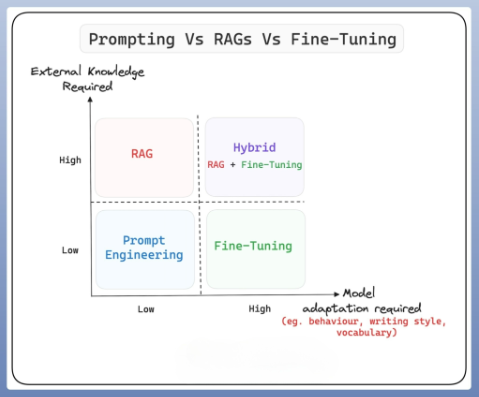
\includegraphics[width=0.85\textwidth,keepaspectratio]{imaxes/5_RAG_RAGvsFineTuning.png}
  \caption[Comparativa RAG vs Fine-Tuning]{Comparativa RAG vs Fine-Tuning. \textit{Fuente: \cite{Celik2023}}}
  \label{fig:5_RAG_RAGvsFineTuning}
\end{figure}


